\documentclass[]{beamer}
\usepackage{tikz}
\geometry{papersize={13cm, 5cm}}
\usetikzlibrary{positioning, arrows.meta}
\beamertemplatenavigationsymbolsempty
\setbeamertemplate{frametitle}[default][center]

\begin{document}
\begin{frame}
    \frametitle{Block Diagram}
    \vspace{0.25cm}
    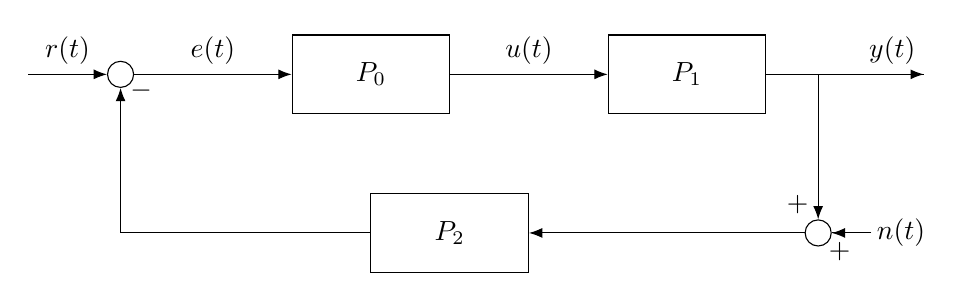
\begin{tikzpicture}[auto, node distance=2cm,>=Latex,
        input/.style = {coordinate},
        output/.style = {coordinate},
        block/.style = {draw, rectangle, minimum height=1cm, minimum width=2cm},
        sum/.style = {draw, circle, node distance=1cm},
        ]
        \node [input](input){};
        \node [sum, right=of input] (sum) {};
        \node [block, right=of sum] (controller) {$P_0$};
        \node [block, right=of controller] (system) {$P_1$};
        \node [output, right= 2cm of system] (output) {};
        \node [block, below left= 1cm and 1cm of system] (feedback) {$P_2$};
        \node [sum, right= 3.5 cm of feedback] (sum2) {};
        \node [input, right= 0.5cm of sum2](input2){};
        
        \draw [->] (input) -- node {$r(t)$} (sum);
        \draw [->] (sum) -- node {$e(t)$} (controller);
        \draw [->] (controller) -- node {$u(t)$} (system);
        \draw [->] (system) -- node [name=y, pos=0.5] {} (output);
        \draw (system) -- node [pos=0.8] {$y(t)$} (output);
        \draw [->] (system) -| (sum2) node[pos=0.95, left] {$+$};
        \draw [->] (feedback) -| node[pos=0.99, right] {$-$} (sum);
        \draw [->] (input2) -- node[right= 0.2cm of input]{$n(t)$} (sum2);
        \draw (input2) -- node[below,pos=0.8]{$+$} (sum2);
        \draw [->] (sum2) -- (feedback);
        
    \end{tikzpicture}
\end{frame}
\begin{frame}
    \frametitle{Block Diagram}
    \vspace{0.25cm}
    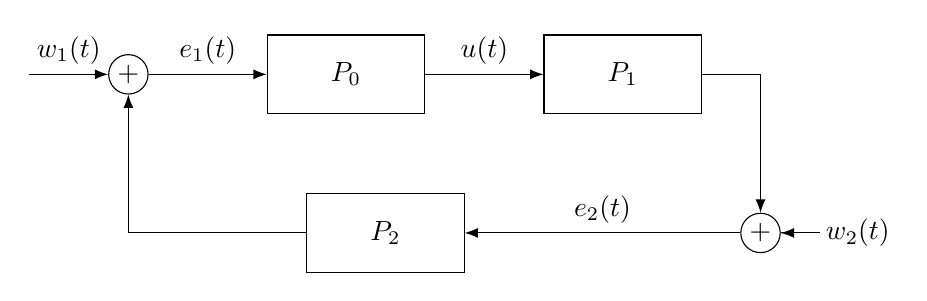
\begin{tikzpicture}[auto, node distance=2cm,>=Latex,
        input/.style = {coordinate},
        output/.style = {coordinate},
        block/.style = {draw, rectangle, minimum height=1cm, minimum width=2cm},
        sum/.style = {draw, circle, node distance=1cm, label=center:$+$, minimum size=0.5cm},
        ]
        \node [input](input){};
        \node [sum, right=of input] (sum) {};
        \node [block, right= 1.5 of sum] (controller) {$P_0$};
        \node [block, right= 1.5of controller] (system) {$P_1$};
        \node [output, right= 2cm of system] (output) {};
        \node [block, below left= 1cm and 1cm of system] (feedback) {$P_2$};
        \node [sum, right= 3.5 cm of feedback] (sum2) {};
        \node [input, right= 0.5cm of sum2](input2){};
        
        \draw [->] (input) -- node {$w_1(t)$} (sum);
        \draw [->] (sum) -- node {$e_1(t)$} (controller);
        \draw [->] (controller) -- node {$u(t)$} (system);
        \draw [->] (system) -| (sum2) node[pos=0.95, left] {};
        \draw [->] (feedback) -| node[pos=0.99, right] {} (sum);
        \draw [->] (input2) -- node[right= 0.2cm of input]{$w_2(t)$} (sum2);
        \draw (input2) -- node[below,pos=0.8]{} (sum2);
        \draw [->] (sum2) -- node[above] {$e_2(t)$} (feedback);
        
    \end{tikzpicture}
\end{frame}
\end{document}